% ======================================================================
% DOCUMENT METADATA - REQUIRED FOR ACCESSIBILITY
% ======================================================================
% This MUST be the first thing in your document, before \documentclass
% It configures the PDF for accessibility compliance
\DocumentMetadata{
  pdfstandard=a-2u,    % PDF/A-2u format (archival standard with Unicode support)
  pdfstandard=ua-1,    % Add PDF/UA-1 accessibility conformance target
  pdfversion=1.7,          % Explicit PDF version used for compatibility with conformance tooling
  lang=en-US,               % Document language (required for screen readers)
  tagging=on,                 % Enable PDF tagging (required for accessibility)
  tagging-setup={
    math/alt/use,                         % Keep math accessibility enabled (screen readers get tagged math)
    math/mathml/AF=false,    % Do not embed MathML as PDF Associated Files (helps some strict conformance checkers)
    math/tex/AF=false,             % Do not embed TeX source as Associated Files
    math/mathml/sources=      % Clear MathML source attachment list (avoid extra embedded helper files)
  }
}

% ======================================================================
% DOCUMENT CLASS
% ======================================================================
% ltx-talk: A presentation document class for accessible slides
%
% What is ltx-talk?
% - Created by the LaTeX Project team as part of the LaTeX Tagging Project
% - Specifically designed to generate accessible PDFs with proper tagging
% - Purpose-built replacement for Beamer that meets WCAG 2.1 Level AA standards
% - Included in TeX Live 2023+ (no separate installation needed)
%
% Migrating from Beamer:
% ✓ SIMILAR: The \begin{frame}...\end{frame} environment structure
% ✗ WON'T WORK: Beamer themes, templates, and setup commands:
%   - \usetheme{}, \usecolortheme{}, \usefonttheme{} (no theme system)
%   - \setbeamertemplate{} commands (different template approach)
%   - \setbeamercolor{}, \setbeamerfont{} (use standard xcolor/fontspec instead)
%   - Navigation symbols, footline templates (ltx-talk uses different methods)
% → You'll need to recreate your styling using standard LaTeX packages
% ✓ GOOD NEWS: This is ONE-TIME PREAMBLE WORK. Create your styling once,
%   then copy this preamble to all future talks. Your frames mostly work as-is!
%
% The [frame-title-arg] option allows frame titles to be passed as arguments
% similar to Beamer: \begin{frame}{Title}
%
% CRITICAL REQUIREMENTS:
% - LaTeX Engine: LuaLaTeX strongly recommended (this template requires it)
%   * pdfLaTeX has partial support but requires manual MathML files
%   * XeLaTeX does NOT support accessibility tagging
% - TeX Distribution: TeX Live 2023 or later with all packages updated
%   * TeX Live 2022 or earlier will NOT work
%   * Update using TeX Live Manager (Windows) or TeX Live Utility (Mac)
% - Overleaf: YES, this works on Overleaf via Overleaf Labs program
%   * Opt in at: https://www.overleaf.com/labs/participate
%   * Enable "Rolling TeX Live releases"
%   * Select "Rolling TeXLive (labs)" in project settings
%   * Set Compiler to LuaLaTeX
\documentclass[frame-title-arg]{ltx-talk}

% ======================================================================
% PACKAGE IMPORTS
% ======================================================================
\usepackage{booktabs}      % Professional-quality tables
\usepackage{xcolor}          % Color support (needed for accessibility-friendly colors)
\usepackage{fancyvrb}      % Enhanced verbatim environment
\usepackage[normalem]{ulem} % Underline support (normalem prevents emphasis from being underlined)

% ======================================================================
% ACCESSIBILITY CONFIGURATION
% ======================================================================
% Configure PDF tagging for accessibility compliance

\ExplSyntaxOn
\AtBeginDocument{
  % Replace ltx-talk's default section-title tagging with "do nothing"
  % (stops Acrobat complaining about empty H1 tags in sections).
  %
  % Problem: ltx-talk uses \section for structural organization in slides,
  % but section titles are often organizational markers only.
  % Some validators complain about empty H1 tags generated for sections.
  %
  % Solution: disable section-title tagging and use H1 on frame titles.
  \NewTaggingSocketPlug { talk / sec / title } { none } { }
  \AssignTaggingSocketPlug { talk / sec / title } { none }
}
\ExplSyntaxOff

% Tag frame titles as H1 headings for proper document structure.
% This works with the section-title suppression above.
\tagpdfsetup{role / new-tag = frametitle / H1}

% ======================================================================
% COLOR DEFINITIONS
% ======================================================================
% Define colors with sufficient contrast for WCAG 2.1 Level AA compliance
% All colors should have at least 4.5:1 contrast ratio with white background

\colorlet{AccessibleRed}{red!80!black}      % Darker red for better contrast
\colorlet{AccessibleGreen}{green!40!black}  % Darker green for WCAG AA compliance (4.5:1 contrast)
\definecolor{AltYellow}{RGB}{255,245,170}   % Soft yellow for highlighting code

% ======================================================================
% CUSTOM COMMANDS FOR TEXT COLORS
% ======================================================================
% Shortcuts for commonly used colors in teaching materials
% Use these to maintain consistent, accessible colors throughout your slides

\newcommand\tb[1]{\textcolor{blue}{#1}}                       % Blue text
\newcommand\tr[1]{\textcolor{AccessibleRed}{#1}}     % Red text (accessible)
\newcommand\tg[1]{\textcolor{AccessibleGreen}{#1}} % Green text (accessible)
% Note: Plain yellow fails WCAG contrast requirements - use AltYellow for backgrounds only

% ======================================================================
% CUSTOM COMMANDS FOR HIGHLIGHTED CODE
% ======================================================================
% \AltBox highlights code snippets with yellow background
% Useful for drawing attention to required accessibility changes in examples

\newcommand{\AltBox}[1]{%
  {\setlength{\fboxsep}{0pt}%
   \colorbox{AltYellow}{\texttt{#1}}}%
}

% ======================================================================
% HYPERLINK CONFIGURATION
% ======================================================================
% Links should be both colored AND underlined for accessibility
% Color alone is not sufficient (fails WCAG guidelines)

\urlstyle{same}  % URLs use the same font as surrounding text

% Custom commands for underlined hyperlinks
\newcommand{\hrefu}[2]{\href{#1}{\uline{#2}}}  % Hyperlink with underline
\newcommand{\urlu}[1]{\uline{\url{#1}}}        % URL with underline

% Set link colors (same color for consistency)
\hypersetup{
  colorlinks=true,
  linkcolor=AccessibleGreen,   % Internal links (TOC, references)
  urlcolor=AccessibleGreen,    % External URLs
  citecolor=AccessibleGreen    % Citations
}

% ======================================================================
% SLIDE FORMATTING - FRAME TITLES
% ======================================================================
% Customize the appearance of slide titles
% Left-justified, large font, blue color for visual emphasis

\EditInstance{frametitle}{header}{
  font  = \LARGE\raggedright,  % Large, left-aligned
  color = blue                  % Blue for consistency with theme
}

% ======================================================================
% SLIDE FORMATTING - FOOTER
% ======================================================================
% Customize footer content:
% - Title slide: logo + author/year
% - Other slides: right-aligned frame number

\makeatletter
\renewcommand\@framenumber{%
  \ifnum\value{page}=1\relax
    % --- title slide footer content ---
    \hspace*{-.2in}%
    \raisebox{0.0in}[.25in][.0in]{
\includegraphics[width=.45in,alt={UC Berkeley Haas School of Business logo}]{BerkeleyHaas}}
    \hfill \hspace*{-.5in} Richard Stanton, \the\year \hfill 
  \else
    % Other slides: frame number only, right-aligned
    \hfill\arabic{frame}%
  \fi
}
\makeatother

\EditInstance{footer}{std}{
  color         = black,
  font          = \tiny,
  left-hspace   = 0.9cm,
  right-hspace  = 0.5cm,
  separator     = \hfill,
  element-order = {framenumber},
}

% ======================================================================
% FONT CONFIGURATION (OPTIONAL)
% ======================================================================
% Font choices that ensure consistency between text and math mode
% This is OPTIONAL and purely for visual consistency - not required for accessibility
%
% These fonts (Lato and LeteSansMath.otf) are included in TeX Live 2023+
% If you get font errors, you can comment out these lines or use different fonts
%
% Why these specific settings?
% - Lining + Monospaced numbers make digits look the same in text and math
% - LeteSansMath matches the Lato sans-serif style
% - This creates visual consistency that improves readability

\setmainfont{Lato}[
  Ligatures=TeX,
  Numbers={Lining,Monospaced}  % Same number style in text and math
]
\setsansfont{Lato}[
  Ligatures=TeX,
  Numbers={Lining,Monospaced}  % Same number style in text and math
]

\setmathfont{LeteSansMath.otf}  % Sans-serif math font to match Lato

% ======================================================================
% DOCUMENT INFORMATION
% ======================================================================
% Define title, author, institution, and date
% These work just like in Beamer

% Keep metadata fields simple; render rich title-page content manually below.
\title{Accessible Slides in LaTeX}
\author{Richard Stanton}
\institute{\small UC Berkeley}
\date{\today}

% ======================================================================
% BEGIN DOCUMENT
% ======================================================================

\begin{document}

% ======================================================================
% TITLE SLIDE
% ======================================================================
% Build the title slide manually so all links/details stay on page 1
% without triggering title-structure tagging warnings.

\begin{frame*}{}
  \centering
  {\LARGE\textcolor{blue}{Accessible Slides in LaTeX}}\\[0.5\baselineskip]
  {\normalsize \urlu{https://github.com/rhstanton/accessible_LaTeX}}\\[1.0\baselineskip]
  {\large Version 1.4}\\[1.0\baselineskip]
  {\normalsize Richard Stanton}\\[0.25\baselineskip]
  {\normalsize \hrefu{mailto:richard.stanton@berkeley.edu}{richard.stanton@berkeley.edu}}\\[0.75\baselineskip]
  {\small UC Berkeley}\\[0.25\baselineskip]
  {\small \today}
\end{frame*}

% Keep title slide unnumbered and start content slide numbering at 1.
\setcounter{frame}{0}

\section{Introduction}

\begin{frame}{Introduction}

\begin{itemize}

\item On January 8, 2026, we were notified by campus that, beginning in April 2026,

  \begin{quotation}
    \color{blue}
``The updated requirements of the ADA require that digital course materials provided to students, even materials inside password-protected course sites like bCourses, will need to comply with accessibility standards (Web Content Accessibility Guidelines (\hrefu{https://www.w3.org/WAI/standards-guidelines/wcag/}{WCAG}) 2.1 Level AA).''
\end{quotation}

\item Many of us use \LaTeX\ to create teaching materials---both slides and documents.
\item Standard \LaTeX\ (including Beamer) does not automatically generate accessible PDFs.
\item \tb{The good news:} The \LaTeX\ Project team has developed solutions!

\end{itemize}
\end{frame}

\begin{frame}{What is this project?}

\begin{itemize}
\item An experiment exploring accessible \LaTeX\ documents using the \LaTeX\ Tagging Project
  \begin{itemize}
  \item \tg{Two templates:} Articles (\texttt{article} class) and slides (\texttt{ltx-talk})
  \item \tg{Shows:} What's common to both, what's different
  \item \tg{Contains:} Working examples with math, text, graphics, and tables
  \item \tg{Scores:} Perfect 100\% from the bCourses accessibility checker (Ally)
  \end{itemize}

\bigskip

\item \tb{How to use it:}
  \begin{enumerate}
  \item \textbf{Learn the common requirements:} Apply to any \LaTeX\ document
  \item \textbf{See class-specific needs:} Understand slides vs. articles
  \item \textbf{Copy and adapt:} Use as templates for your documents
  \item \textbf{Study the code:} Heavily commented for learning
  \end{enumerate}

\bigskip

\item Available at: \urlu{https://github.com/rhstanton/accessible_LaTeX}
  
\end{itemize}
\end{frame}

\begin{frame}{Converting to accessible LaTeX: Overview}

\begin{itemize}
\item {\color{AccessibleGreen}\textbf{Your existing \LaTeX\ skills transfer}} - you're just adding accessibility features
\item {\color{AccessibleGreen}\textbf{The changes are minimal}} and follow consistent patterns

\bigskip

\item \textbf{Common requirements} (both slides \& articles):
  \begin{itemize}
  \item Add document metadata and enable PDF tagging
  \item Tag images with alt text; tag table headers
  \item Use accessible colors; compile with LuaLaTeX
  \end{itemize}

\bigskip

\item \textbf{Key difference:}
  \begin{itemize}
  \item Articles: {\color{AccessibleGreen}Keep your existing class!} Just add accessibility features
  \item Slides: Switch to \texttt{ltx-talk} (similar syntax, but recreate styling)
  \end{itemize}

\bigskip

\item Both require LaTeX kernel 2025-11-01 or later (see next slides for details)
\item {\color{blue}See ``Getting started'' slides at end for detailed steps}
\item \hrefu{https://latex3.github.io/tagging-project/documentation/usage-instructions}{LaTeX Tagging Project documentation}

\end{itemize}
\end{frame}

\begin{frame}{TeX version requirements (both slides and articles)}

\begin{itemize}
\item \tg{Minimum:} TeX Live 2023 or later with all packages updated
\item \tg{Critical:} Must have LaTeX kernel 2025-11-01 or later
  \begin{itemize}
  \item Update via TeX Live Manager (Windows) or TeX Live Utility (Mac)
  \item Or use Overleaf Labs (see next slide)
  \end{itemize}
\item \tr{Will NOT work:} TeX Live 2022 or earlier

\end{itemize}
\end{frame}

\begin{frame}{\tb{You \textbf{CAN} use Overleaf (both slides and articles)}}

\begin{itemize}
\item \texttt{ltx-talk} requires a very recent TeX Live version
\item This is available through Overleaf's \tb{Labs program} (not standard Overleaf)
  
\bigskip

\item \textbf{\tb{Using Overleaf (2 steps)}}
  \begin{enumerate}
  \item \textbf{Join Overleaf Labs}: 
    \begin{itemize}
    \item Visit \urlu{https://www.overleaf.com/labs/participate}
    \item Opt in and enable ``Rolling TeX Live releases''
    \end{itemize}
  \item \textbf{Configure project}:
    \begin{itemize}
    \item Set TeX Live version to \tg{``Rolling TeXLive (labs)''} (bottom of list)
    \item Set Compiler to \tg{LuaLaTeX}
    \end{itemize}
  \end{enumerate}
  
\bigskip

\item \textbf{Resources}: \urlu{https://docs.overleaf.com/writing-and-editing/creating-accessible-pdfs}

\end{itemize}
\end{frame}

\begin{frame}{Common requirements (1/3): Document Metadata}

\bigskip

\begin{itemize}
\item \tb{\textbf{REQUIRED for both slides AND articles}}

\bigskip

\item Every accessible document \tr{must} begin with \texttt{\textbackslash DocumentMetadata}
\item Goes \emph{before} \texttt{\textbackslash documentclass}

\bigskip

\fbox{%
\begin{minipage}{0.9\linewidth}
\ttfamily\scriptsize
\textbackslash DocumentMetadata\{\\[0.5ex]
\hspace*{0.2in}pdfstandard=a-2u,\hspace*{0.425in}\% PDF/A-2u format\\[0.5ex]
\hspace*{0.2in}pdfstandard=ua-1,\hspace*{0.42in}\% Add PDF/UA-1 conformance target\\[0.5ex]
\hspace*{0.2in}pdfversion=1.7,\hspace*{0.55in}\% Explicit PDF version\\[0.5ex]
\hspace*{0.2in}lang=en-US,\hspace*{0.78in}\% Language for screen readers\\[0.5ex]
\hspace*{0.2in}tagging=on,\hspace*{0.78in}\% Enable PDF tagging\\[0.5ex]
\hspace*{0.2in}tagging-setup=\{\\[0.5ex]
\hspace*{0.4in}math/alt/use,\hspace*{0.5in}\% Keep math accessibility enabled\\[0.5ex]
\hspace*{0.4in}math/mathml/AF=false,\hspace*{0.03in}\% Do not embed MathML as PDF Associated Files\\[0.5ex]
\hspace*{0.4in}math/tex/AF=false,\hspace*{0.2in}\% Do not embed TeX source as Associated Files\\[0.5ex]
\hspace*{0.4in}math/mathml/sources=\hspace*{0.08in}\% Clear MathML source attachment list\\[0.5ex]
\hspace*{0.2in}\}\\[0.5ex]
\}
\end{minipage}
}

\bigskip

\item Configures accessibility, math tagging, and validator-compatibility behavior in one place.
  
\end{itemize}
\end{frame}

\begin{frame}{Common requirements (2/3): Images, Tables and Colors}

  \bigskip
  
\begin{itemize}
\item \tb{\textbf{REQUIRED for both slides AND articles}}

\bigskip

\item \textbf{Images:} All images must include alt text descriptions
  \begin{itemize}
  \item Allows screen readers to describe visual content
  \item Even decorative images need marking
  \item See dedicated ``Figures'' slide for examples
  \end{itemize}

\bigskip

\item \textbf{Tables:} Must specify which rows are headers
  \begin{itemize}
  \item Helps screen readers navigate table structure
  \item Essential for data accessibility
  \item See dedicated ``Tables'' slide for examples
  \end{itemize}

\bigskip  
  
\item \textbf{Accessible colors:} WCAG 2.1 requires 4.5:1 contrast ratio
\medskip  

\fbox{%
\begin{minipage}{0.9\linewidth}
\ttfamily\small
\textbackslash colorlet\{AccessibleRed\}\{red!80!black\}\\[0.5ex]
\textbackslash colorlet\{AccessibleGreen\}\{green!40!black\}\\[0.5ex]
\% Standard blue is fine as-is
\end{minipage}
}

  
\end{itemize}
\end{frame}

\begin{frame}{Common requirements (3/3): LuaLaTeX}

\begin{itemize}
\item \tb{\textbf{REQUIRED for both slides AND articles}}

\bigskip

\item You \tr{must} compile with LuaLaTeX (not pdfLaTeX or XeLaTeX)

\bigskip

\item \textbf{Why LuaLaTeX?}
  \begin{enumerate}
  \item \textbf{Automatic MathML:} Makes math accessible without manual work
  \item \textbf{Full tagging support:} Complete PDF accessibility features
  \item \textbf{Modern fonts:} Handles Unicode and OpenType fonts
  \end{enumerate}

\bigskip

\item \textbf{How to switch:}
  \begin{itemize}
  \item Command line: \texttt{lualatex filename.tex}
  \item Most editors: Select ``LuaLaTeX'' from compiler menu
  \end{itemize}

\end{itemize}
\end{frame}

\begin{frame}{The basics}
  \begin{itemize}
  \item Slides are put inside a \texttt{frame} environment, just like in Beamer.
  \item So \textbf{\color{blue}existing source files don't need a lot of editing.}
  \item Here's some gratuitous  $\mathit{math}$ for the accessibility checker.
  \end{itemize}
  
\vspace*{0.25in}
    
\fbox{%
\begin{minipage}{0.95\linewidth}
\ttfamily\small
\textbackslash begin\{frame\}\{The basics\}\\
\textbackslash begin\{itemize\}\\
\textbackslash item Slides are put inside a \textbackslash texttt\{frame\} environment, just like in Beamer.\\
\textbackslash item So \textbackslash textbf\{\textbackslash color\{blue\}existing source files don't need a lot of editing.\}\\
\textbackslash item Here's some gratuitous  \$\textbackslash mathit\{math\}\$ for the accessibility checker.\\
\textbackslash end\{itemize\}\\
\textbackslash end\{frame\}
\end{minipage}
}

\vspace*{0.25in}

\begin{itemize}
\item \tb{Note:} I set the fonts in this file so that numbers, percent signs, and dollar signs look the same in both math and text mode (my pet Beamer peeve\ldots)
    \begin{itemize}
    \item {\color{AccessibleRed} Text:}  \$1234567890\%.
    \item {\color{AccessibleRed} Math:}  $\$1234567890\%.$
    \end{itemize}
  \end{itemize}
\end{frame}

% ======================================================================
% NOTE: frame* (with asterisk) creates an UNNUMBERED slide
% Use frame* when you don't want the slide number to increment
% (e.g., for subsidiary slides or examples that break up the flow)
% ======================================================================
\begin{frame*}{Figures}

\vspace*{.2in}

\begin{itemize}
\item Including figures is the same as in Beamer (e.g., using \texttt{\textbackslash includegraphics}),
but you need to provide a \tr{text description}.

\vspace*{0.25in}

\fbox{%
  \ttfamily\small
  \textbackslash includegraphics[height=.4\textbackslash textheight,%
  \AltBox{alt=\{A capybara\}}%
  ]\{capybara.jpg\}%
}

\end{itemize}

\vspace*{0.25in}

\centering
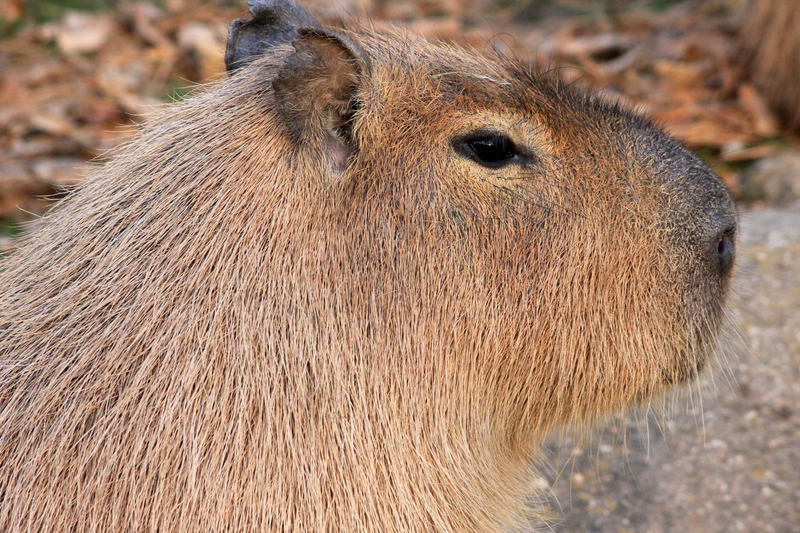
\includegraphics[height=.5\textheight, alt={A capybara}]{capybara.jpg}

\end{frame*}

\begin{frame}{Tables}

\small  
\begin{itemize}
\item Including tables is the same as in Beamer (e.g., using the \texttt{tabular} environment).
\item  Also need to specify \tr{header rows}.  Use \texttt{\{1\}} for 1 header row, \texttt{\{1,2\}} for 2 rows, etc.
\item  \textbf{Note:} This example may still trigger PAC's \texttt{Table header cell has no associated subcells} warning even when the source tagging is correct.
  
\vspace*{0.05in}
    
\fbox{%
\begin{minipage}{0.95\linewidth}
\ttfamily\footnotesize
\AltBox{\textbackslash tagpdfsetup\{table/header-rows=\{1,2,3\}\}} \\
\textbackslash begin\{tabular\}\{ccccrcccr\} \\
\textbackslash toprule \\
\textrm{\color{blue}\footnotesize $\leftarrow$ 3 header rows} \\
\textbackslash midrule \\
\textrm{\color{AccessibleGreen}\footnotesize $\leftarrow$ data rows} \\
\textbackslash bottomrule \\
\textbackslash end\{tabular\}
\end{minipage}
}

\end{itemize}

\vspace*{0.05in}
  
\begin{center}\scriptsize
\tagpdfsetup{table/header-rows={1,2,3}}
  \begin{tabular}{ccccrcccr}
  \toprule
  \color{blue} & \color{blue} & \color{blue} & \color{blue} & \multicolumn{1}{c}{\color{blue}Days} & \color{blue}Days in & \color{blue} & \color{blue} & \color{blue}\\
\color{blue}Payment & \color{blue}Caplet & \color{blue} & \color{blue}Forward & \multicolumn{1}{c}{\color{blue}to} & \color{blue}accrual & \color{blue} & \color{blue}\\
  \color{blue}date & \color{blue}expiry date & \color{blue}$DF_\text{pay}$ & \color{blue}rate & \multicolumn{1}{c}{\color{blue}expiry} & \color{blue}period & \color{blue}$T_\text{expiry}$ & \color{blue}$\Delta$ & \multicolumn{1}{c}{\color{blue}Caplet} \\
\midrule
  \color{AccessibleGreen}2004/12/01 & \color{AccessibleGreen}--- & \color{AccessibleGreen}0.99550 & \color{AccessibleGreen}0.01790 & \color{AccessibleGreen}0 & \color{AccessibleGreen}91 & \color{AccessibleGreen}0.00000 & \color{AccessibleGreen}0.25278 & \color{AccessibleGreen}--- \hspace*{0.15in}\\
  \color{AccessibleGreen}2005/03/01 & \color{AccessibleGreen}2004/11/29 & \color{AccessibleGreen}0.99008 & \color{AccessibleGreen}0.02188 & \color{AccessibleGreen}89 & \color{AccessibleGreen}90 & \color{AccessibleGreen}0.24384 & \color{AccessibleGreen}0.25000 & \color{AccessibleGreen}1,178.77\\
  \color{AccessibleGreen}2005/06/01 & \color{AccessibleGreen}2005/02/25 & \color{AccessibleGreen}0.98401 & \color{AccessibleGreen}0.02413 & \color{AccessibleGreen}177 & \color{AccessibleGreen}92 & \color{AccessibleGreen}0.48493 & \color{AccessibleGreen}0.25556 & \color{AccessibleGreen}4,844.73\\
  \color{AccessibleGreen}2005/09/01 & \color{AccessibleGreen}2005/05/27 & \color{AccessibleGreen}0.97733 & \color{AccessibleGreen}0.02675 & \color{AccessibleGreen}268 & \color{AccessibleGreen}92 & \color{AccessibleGreen}0.73425 & \color{AccessibleGreen}0.25556 & \color{AccessibleGreen}10,016.71\\
  \bottomrule
\end{tabular}  
\end{center}

\end{frame}

\begin{frame}{Common pitfalls}
  \begin{itemize}
  \item \tr{Forgetting alt text for images}
    \begin{itemize}
    \item Every \texttt{\textbackslash includegraphics} needs an \texttt{alt=\{...\}} parameter
    \item Even decorative images need alt text (use \texttt{alt=\{decorative\}})
    \end{itemize}
    
  \item \tr{Not specifying table header rows}
    \begin{itemize}
    \item Add \texttt{\textbackslash tagpdfsetup\{table/header-rows=\{...\}\}} before each table
    \item Use \texttt{\{1\}} for 1 header row, \texttt{\{1,2\}} for 2 header rows, etc.
    \end{itemize}
    
  \item \tr{Insufficient color contrast}
    \begin{itemize}
    \item WCAG 2.1 requires 4.5:1 contrast ratio for normal text
    \item Avoid light colors: \texttt{yellow}, \texttt{cyan} fail contrast requirements
    \item Darken \texttt{red} and \texttt{green}: use \texttt{red!80!black}, \texttt{green!40!black}
    \item Standard \texttt{blue} is fine and meets WCAG requirements
    \item Test with a contrast checker: \urlu{https://webaim.org/resources/contrastchecker/}
    \end{itemize}

  \item \tr{Using the wrong compiler}
    \begin{itemize}
    \item Make sure your editor is set to use \tg{LuaLaTeX}, not \tr{pdfLaTeX}
    \end{itemize}
    
  \item \tr{Old TeX distribution}
    \begin{itemize}
    \item TeX Live 2022 or earlier won't work
    \item Update packages using TeX Live Manager (Windows) or TeX Live Utility (Mac)
    \end{itemize}
    
  \end{itemize}
\end{frame}

\begin{frame}{Getting started: Common steps}
  \begin{enumerate}
  \item \textbf{Setup environment:} Use Overleaf Labs OR install/update TeX Live locally
    \begin{itemize}
    \item Overleaf: See earlier slides for Labs setup
    \item Local: Update via TeX Live Manager/Utility
    \end{itemize}
  \item \textbf{Get templates:} Download from \urlu{https://github.com/rhstanton/accessible_LaTeX}
  \item \textbf{Add accessibility features:}
    \begin{itemize}
    \item Add \texttt{alt} text to images
    \item Add \texttt{table/header-rows} to tables
    \end{itemize}
  \item \textbf{Set compiler to LuaLaTeX}
  \item \textbf{Compile:}
    \begin{itemize}
    \item Compile with LuaLaTeX
    \item PDF file now scores 100\% on \tb{Ally}
    \end{itemize}
  \end{enumerate}
\end{frame}

\begin{frame}{Getting started: What's different by document type}

\bigskip  
  
  \textbf{\tb{Articles} (using \texttt{article}, \texttt{report}, \texttt{book}, etc.):}
  \begin{itemize}
  \item Add \texttt{\textbackslash DocumentMetadata} before \texttt{\textbackslash documentclass}
  \item Include the \texttt{tagging-setup} block in \texttt{\textbackslash DocumentMetadata} (as shown in this template)
  \item Switch to \texttt{fontspec} and \texttt{unicode-math} packages
  \item \tg{Keep your existing documentclass!}
  \end{itemize}

\bigskip

  \textbf{\tr{Slides} (migrating from Beamer):}
  \begin{itemize}
  \item Copy preamble from \texttt{accessible\_slides.tex}
  \item Change \texttt{\textbackslash documentclass\{beamer\}} to \texttt{\textbackslash documentclass[frame-title-arg]\{ltx-talk\}}
  \item \tr{Remove Beamer themes/templates/colors}
  \item \tg{Recreate styling} using standard LaTeX/xcolor
  \item \tg{One-time preamble work}—then reuse for all future talks!
  
\bigskip

  \item Questions? \hrefu{mailto:richard.stanton@berkeley.edu}{richard.stanton@berkeley.edu}
  \end{itemize}
\end{frame}

\begin{frame}{Validation workflow: use multiple checkers}

\begin{itemize}
\item No single checker catches everything.
\item Accessibility usability checks and strict PDF conformance checks are not identical.
\item A practical workflow is to run more than one checker and compare findings.

\bigskip

\item \textbf{Checkers used so far}
  \begin{itemize}
  \item \tb{Ally} (built into bCourses)
  \item \tb{veraPDF} (open-source PDF conformance validator, \urlu{https://verapdf.org/})
  \item \tb{PAC} (PDF Accessibility Checker, \urlu{https://pac.pdf-accessibility.org/})
  \item \tb{Adobe Acrobat}.
  \end{itemize}
\end{itemize}

\end{frame}

\begin{frame}{Optional validator cleanup step: \texttt{strip\_af.py}}

\begin{itemize}
\item The metadata settings alone are enough to generate a 100\% score on Ally.
\item Stricter checkers (e.g., \tr{veraPDF}) may still complain about /AF or embedded-file structures.
\item To remove these and stop the complaints, run \texttt{strip\_af.py}:

\bigskip

\fbox{%
\begin{minipage}{0.9\linewidth}
\ttfamily
python strip\_af.py build/accessible\_slides.pdf
\end{minipage}
}

\bigskip

\item Prerequisite: install the Python package \tg{pikepdf} first: \texttt{python -m pip install pikepdf}.
\item Then validate \texttt{build/accessible\_slides.pdf} with \texttt{veraPDF}.
\end{itemize}

\end{frame}

\begin{frame}{Validator-specific notes}
  \begin{itemize}
  \item \textbf{Acrobat: ``Lbl and LBody -- Failed'' (validator bug)}
    \begin{itemize}
    \item Appears around figure captions, section numbers, table captions
    \item \tg{This is an Acrobat bug}, not a source error -- \tb{safe to ignore}
    \item The \texttt{<Lbl>} tag is correctly used for numbering
    \item Acrobat's checker incorrectly expects it only in lists
    \item Reference: \urlu{https://tex.stackexchange.com/a/709655/2388}
    \end{itemize}
  
  \item \textbf{PAC table warning (known behavior)}
    \begin{itemize}
    \item PAC can report \texttt{Table header cell has no associated subcells} even when \texttt{table/header-rows} is correct
    \item This behavior is documented by the LaTeX Tagging Project: \urlu{https://github.com/latex3/tagging-project/issues/1056}
    \end{itemize}

  \item \textbf{When this warning appears}
    \begin{itemize}
    \item First confirm source markup is correct (especially \texttt{table/header-rows})
    \item Keep the source tagging and document the validator warning
    \item Report minimal reproductions to tool vendors when possible
    \end{itemize}

\item \textbf{Bottom line}
    \begin{itemize}
    \item Use multiple validators (Ally, veraPDF, PAC, Acrobat) and compare findings
    \item Treat one-tool warnings as signals to investigate, not proof of errors
    \end{itemize}
  \end{itemize}
\end{frame}

\end{document}

% ======================================================================
% EMACS/AUCTEX LOCAL VARIABLES (Optional - for Emacs users only)
% ======================================================================
% The section below configures Emacs/AUCTeX to use the correct LaTeX engine
% and options when compiling this file from within Emacs.
%
% If you use Emacs/AUCTeX: These settings ensure LuaLaTeX is used automatically
% If you use a different editor: You can safely ignore or delete this section
%
% Key settings explained:
%   - TeX-engine: luatex           -> Forces LuaLaTeX (STRONGLY RECOMMENDED!)
%   - TeX-command-extra-options    -> Adds -interaction=nonstopmode flag
%   - TeX-master: t                -> This file is its own master document
%   - eval: commands               -> Custom Emacs functions for this file
%
% IMPORTANT: This template requires LuaLaTeX for automatic MathML generation
% Using pdflatex will require manual MathML files (tedious and error-prone)
%
% For other editors (TeXShop, TeXworks, Overleaf, VS Code, etc.):
% Configure them manually to use LuaLaTeX with -interaction=nonstopmode

%%% Local Variables:
%%% mode: latex
%%% TeX-engine: luatex
%%% TeX-command-extra-options: "-interaction=nonstopmode"
%%% TeX-master: t
%%% eval: (setq-local TeX-command-list (cons '("LatexMk (build)" "latexmk -lualatex -interaction=nonstopmode -file-line-error -synctex=1 -shell-escape -outdir=build %s" TeX-run-TeX nil t :help "Run LatexMk with LuaLaTeX") (remove-if (lambda (x) (equal (car x) "LatexMk (build)")) TeX-command-list)))
%%% eval: (setq org-format-latex-header "\\documentclass[10pt]{RSorg}\\pagestyle{empty}")
%%% eval: '(hide-latex-preamble)
%%% eval: (outline-hide-body)
%%% End:
